\documentclass{beamer}
\usetheme{Montpellier}

\usepackage{color}
\usepackage{amsfonts}
\usepackage{comment}

%%% Al parecer necesito esto en ubuntu para los acentos
%\usepackage[spanish]{babel}
%\selectlanguage{spanish}
%\usepackage[utf8]{inputenc}

\definecolor{myblue}{rgb}{0.25, 0, 0.75}
\definecolor{mygold}{rgb}{1,0.8,0.2}
\definecolor{gray}{rgb}{0.5, 0.5, 0.5}
\definecolor{lucia}{rgb}{0.8,0.4,0.7} 

\newcommand{\myurl}[1]{\href{http://#1}{\textcolor{gray}{\texttt{#1}}}}
\newcommand{\myem}[1]{\structure{#1}}
\newcommand{\myurlshort}[2]{\href{http://#1}{\textcolor{gray}{\textsf{#2}}}}

\newcommand{\RPackage}[1]{\textcolor{gray}{\textsf{#1}}}
\newcommand{\pl}[1]{\texttt{#1}}
\newcommand{\RCode}[1]{\texttt{#1}}
\newcommand{\RFunction}[1]{\textsf{#1}}
\newcommand{\RClass}[1]{\textcolor{mygold}{\textsf{#1}}}
\newcommand{\BIOCfunction}[1]{\textcolor{orange}{#1}}

\setbeamercolor{example text}{fg=lucia}
\setbeamertemplate{sections/subsections in toc}[ball unumbered]
\setbeamertemplate{frametitle continuation}[from second][]
\setbeamertemplate{itemize subitem}[triangle]
\setbeamertemplate{footline}[page number]
\setbeamertemplate{caption}[numbered]
\setbeamertemplate{navigation symbols}{}

\renewcommand{\footnotesize}{\fontsize{6.10}{12}\selectfont}

\def\argmax{\operatornamewithlimits{arg\,max}}
\def\argmin{\operatornamewithlimits{arg\,min}}

%%\bibliographystyle{plain}


\title{Seminar III: R/Bioconductor}
\author{Leonardo Collado Torres \\ lcollado@lcg.unam.mx \\  Bachelor in Genomic Sciences \\ \myurl{www.lcg.unam.mx/\string~lcollado/}}
\date{
August - December, 2009
}








\usepackage{Sweave}
\begin{document}

\begin{frame}[allowframebreaks]
  \titlepage
\end{frame}

\section*{Class outline}

\begin{frame}[allowframebreaks]
  \frametitle{A Case Study with GOs}
  \tableofcontents[hideallsubsections]
\end{frame}

%%%%%%%%%%%%%%%%%%%%%%%%%%%%%%%%%%%%%%%%%%%%%%%%%%%%%%%%%%%%%%%%%%%%%%%%%%%
\section{Intro}

\begin{frame}[allowframebreaks, fragile]
  \frametitle{Packages we'll use today}
  \begin{itemize}
  \item You'll probably need to install a few using \BIOCfunction{biocLite}.
\begin{Schunk}
\begin{Sinput}
> library("ALL")
> library("Biobase")
> library("annotate")
> library("hgu95av2.db")
> library("genefilter")
> library("annaffy")
> library("GO.db")
> library("GOstats")
> library("biomaRt")
> library("hgu133a.db")
> library("lattice")
\end{Sinput}
\end{Schunk}
  \end{itemize}
\end{frame}

%%%%%%%%%%%%%%%%%%%%%%%%%%%%%%%%%%%%%%%%%%%%%%%%%%%%%%%%%%%%%%%%%%%%%%%%%%%
\section{Data and filtering}

\begin{frame}[allowframebreaks, fragile]
  \frametitle{To start off}
  \begin{itemize}
  \item Similar to the 2nd homework, lets create a subset from the \pl{ALL} dataset.
  \item Remember that we are working with leukemia samples and the molecular types BCR/ABL and ALL/AF4 are different translocations.
\begin{Schunk}
\begin{Sinput}
> library("ALL")
> data("ALL")
> types <- c("ALL1/AF4", "BCR/ABL")
> bcell <- grep("^B", as.character(ALL$BT))
> ALL_af4bcr <- ALL[, intersect(bcell, 
+     which(ALL$mol.biol %in% types))]
> ALL_af4bcr$mol.biol <- factor(ALL_af4bcr$mol.biol)
\end{Sinput}
\end{Schunk}
  \item How many features does our subset have?
  \item Samples?
  \end{itemize}
\end{frame}

\begin{frame}[allowframebreaks, fragile]
  \frametitle{Filtering}
  \begin{itemize}
  \item We can make a table to check how many samples we have:
\begin{Schunk}
\begin{Sinput}
> table(ALL_af4bcr$mol.biol)
\end{Sinput}
\begin{Soutput}
ALL1/AF4  BCR/ABL 
      10       37 
\end{Soutput}
\end{Schunk}
  \item Our groups are rather different in size, so the outliers of BCR/ABL will dominate the variance.
  \item There are several options on how to filter the data, but we'll use the 10\% and 90\% quantiles.
  \item How do you find that range?
  \end{itemize}
\end{frame}

\begin{frame}[allowframebreaks, fragile]
  \frametitle{Filtering II}
  \begin{itemize}
  \item Lets take advantage of the \BIOCfunction{quantile} and \BIOCfunction{diff} functions:
\begin{Schunk}
\begin{Sinput}
> qrange <- function(x) diff(quantile(x, 
+     c(0.1, 0.9)))
\end{Sinput}
\end{Schunk}
  \item Now we can use the \pl{nsFilter} function from the \pl{genefilter} package:
\begin{Schunk}
\begin{Sinput}
> suppressWarnings(library("genefilter"))
> library("hgu95av2.db")
> filt_af4bcr <- nsFilter(ALL_af4bcr, 
+     require.entrez = TRUE, require.GOBP = TRUE, 
+     var.fun = qrange, var.cutoff = 0.5)
> ALLfilt_af4bcr <- filt_af4bcr$eset
\end{Sinput}
\end{Schunk}
  \item Previously we had used the \pl{IQR} function instead of our homemade \pl{qrange}.
  \end{itemize}
\end{frame}

\begin{frame}[allowframebreaks, fragile]
  \frametitle{Top 100}
  \begin{itemize}
  \item Now lets find the top 100 genes by carrying out a two group comparison.
  \item We'll need to load some packages first:
\begin{Schunk}
\begin{Sinput}
> library("Biobase")
> library("annotate")
\end{Sinput}
\end{Schunk}
  \item Now we can use the \BIOCfunction{rowttests} function:
\begin{Schunk}
\begin{Sinput}
> rt <- rowttests(ALLfilt_af4bcr, 
+     "mol.biol")
> names(rt)
\end{Sinput}
\begin{Soutput}
[1] "statistic" "dm"        "p.value"  
\end{Soutput}
\end{Schunk}
  \end{itemize}
\end{frame}

\begin{frame}[allowframebreaks]
  \frametitle{Quick exercises}
  Create a histogram of
  \begin{itemize}
  \item the statistic
  \item the p values
  \end{itemize}
\end{frame}

\begin{frame}[fragile, allowframebreaks]
  \frametitle{Solution I}
\begin{Schunk}
\begin{Sinput}
> hist(rt$statistic, breaks = 100, 
+     col = "skyblue")
\end{Sinput}
\end{Schunk}
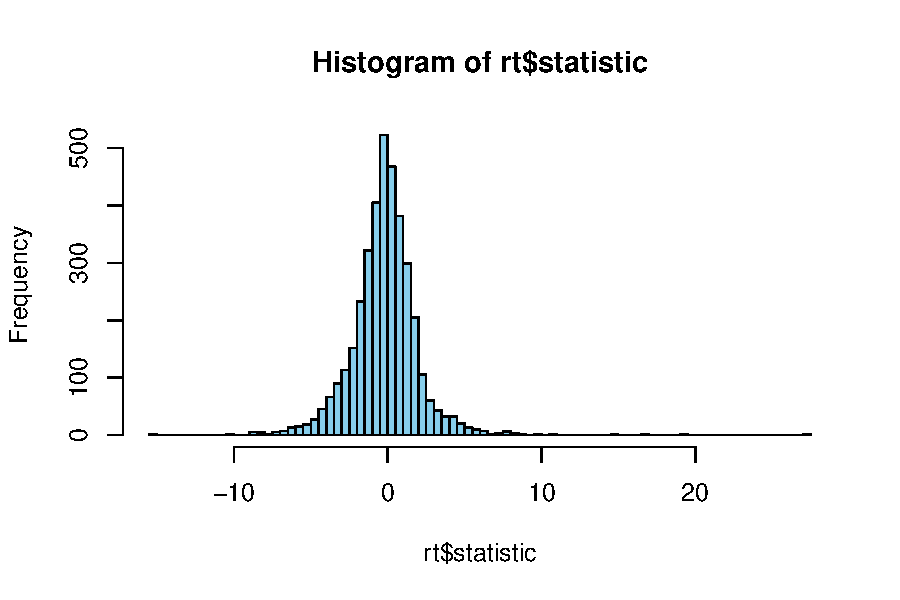
\includegraphics{plots/fig-009}
\end{frame}

\begin{frame}[fragile, allowframebreaks]
  \frametitle{Solution II}
\begin{Schunk}
\begin{Sinput}
> hist(rt$p.value, breaks = 100, 
+     col = "mistyrose")
\end{Sinput}
\end{Schunk}
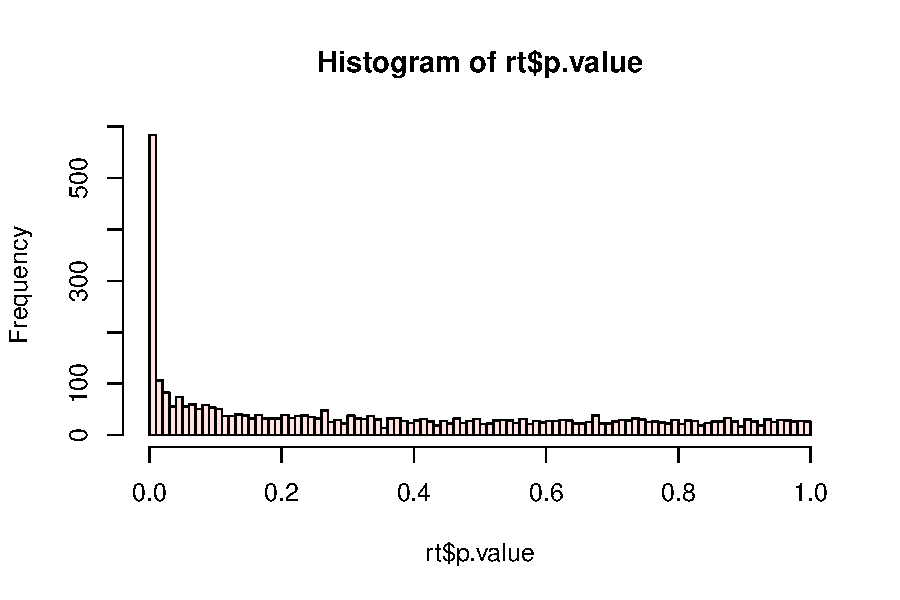
\includegraphics{plots/fig-010}
\end{frame}

\begin{frame}[allowframebreaks, fragile]
  \frametitle{Lowest 400 p values}
  \begin{itemize}
  \item Lets create the \pl{ALLsub} \emph{ExpressionSet} with the 400 probe sets with the lowest p values.
  \item Any ideas?
  \end{itemize}
\end{frame}

\begin{frame}[allowframebreaks, fragile]
  \frametitle{Solution}
  \begin{itemize}
  \item Here is one way:
\begin{Schunk}
\begin{Sinput}
> sel <- order(rt$p.value)[1:400]
> ALLsub <- ALLfilt_af4bcr[sel, ]
\end{Sinput}
\end{Schunk}
  \item Next, lets find how many probe sets in ALL and how many in ALLsub map to the same EntrezGene ID.
  \end{itemize}
\end{frame}

\begin{frame}[allowframebreaks, fragile]
  \frametitle{A trick}
  \begin{itemize}
  \item First lets get the IDs into two separate vectors:
\begin{Schunk}
\begin{Sinput}
> EG <- as.character(hgu95av2ENTREZID[featureNames(ALL)])
> EGsub <- as.character(hgu95av2ENTREZID[featureNames(ALLsub)])
\end{Sinput}
\end{Schunk}
  \item Next, lets use a little trick: using two table functions!
\begin{Schunk}
\begin{Sinput}
> head(table(EG))
\end{Sinput}
\begin{Soutput}
EG
   10   100  1000 10000 10001 10002 
    1     2     2     1     3     2 
\end{Soutput}
\begin{Sinput}
> table(table(EG))
\end{Sinput}
\begin{Soutput}
   1    2    3    4    5    6    7    8 
6891 1495  468   97   25   13    5    5 
   9 
   1 
\end{Soutput}
\begin{Sinput}
> table(table(EGsub))
\end{Sinput}
\begin{Soutput}
  1 
400 
\end{Soutput}
\end{Schunk}
  \item Why do all the probe sets in ALLsub map to a unique EntrezGene ID?
  \end{itemize}
\end{frame}

\begin{frame}[allowframebreaks, fragile]
  \frametitle{Looking at a gene}
  \begin{itemize}
  \item Now lets look at the expression profile of a given gene, for example, CD44.
  \item First, lets find out which features belong to our gene:
\begin{Schunk}
\begin{Sinput}
> syms <- as.character(hgu95av2SYMBOL[featureNames(ALLsub)])
> whFeat <- names(which(syms == "CD44"))
\end{Sinput}
\end{Schunk}
  \item Now lets create a subset of ALLsub with the info we want:
\begin{Schunk}
\begin{Sinput}
> ordSamp <- order(ALLsub$mol.biol)
> CD44 <- ALLsub[whFeat, ordSamp]
\end{Sinput}
\end{Schunk}
  \item What kind of plot should we make to visualize the expression profile of CD44?
  \end{itemize}
\end{frame}

\begin{frame}[fragile, allowframebreaks]
  \frametitle{Simple plot}
  A simple plot is enough:
\begin{Schunk}
\begin{Sinput}
> plot(as.vector(exprs(CD44)), main = whFeat, 
+     col = c("sienna", "tomato")[CD44$mol.biol], 
+     pch = c(15, 16)[CD44$mol.biol], 
+     ylab = "expression")
\end{Sinput}
\end{Schunk}
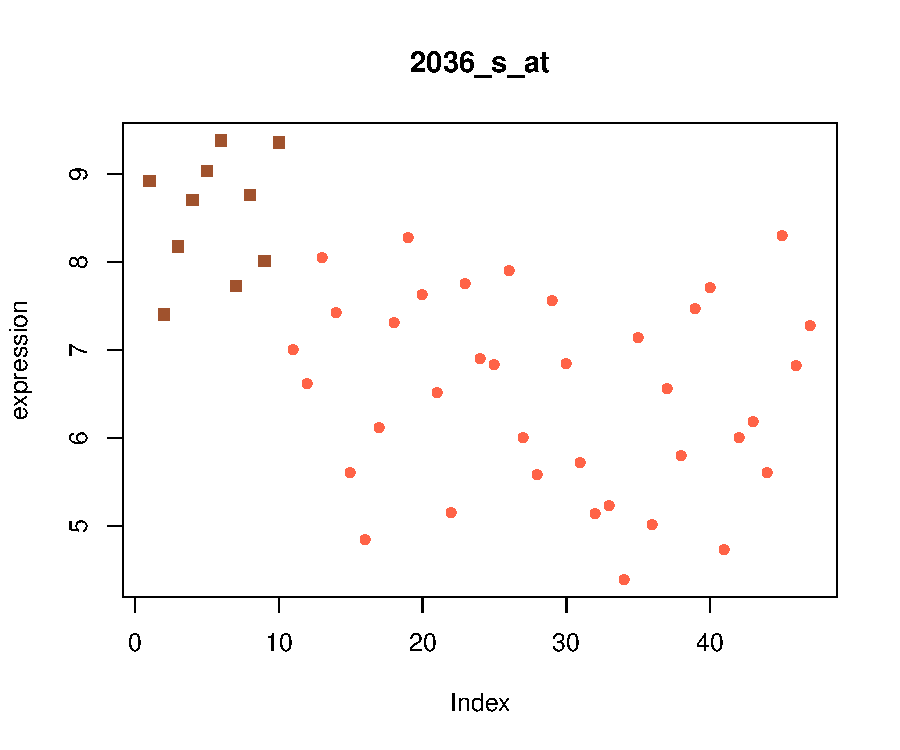
\includegraphics{plots/fig-016}
\end{frame}

\begin{frame}[fragile, allowframebreaks]
  \frametitle{Now a barplot}
  We used some mapping tricks to distinguis the two molecular types. \\ Looks like ALL1/AF4 have higher values than BCR/ABL. \\ Now lets make a barplot to group the values per chromosome:
\begin{Schunk}
\begin{Sinput}
> z <- toTable(hgu95av2CHR[featureNames(ALLsub)])
> chrtab <- table(z$chromosome)
> chrtab
\end{Sinput}
\begin{Soutput}
 1 10 11 12 13 14 15 16 17 18 19  2 20 
43 23 23 20  9 20  5 12 17  6 14 26  9 
21 22  3  4  5  6  7  8  9  X  Y 
 7 13 18 14 11 39 22 14 20 15  1 
\end{Soutput}
\begin{Sinput}
> chridx <- sub("X", "23", names(chrtab))
> chridx <- sub("Y", "24", chridx)
> barplot(chrtab[order(as.integer(chridx))], 
+     cex.names = 0.5, col = rainbow(24))
\end{Sinput}
\end{Schunk}
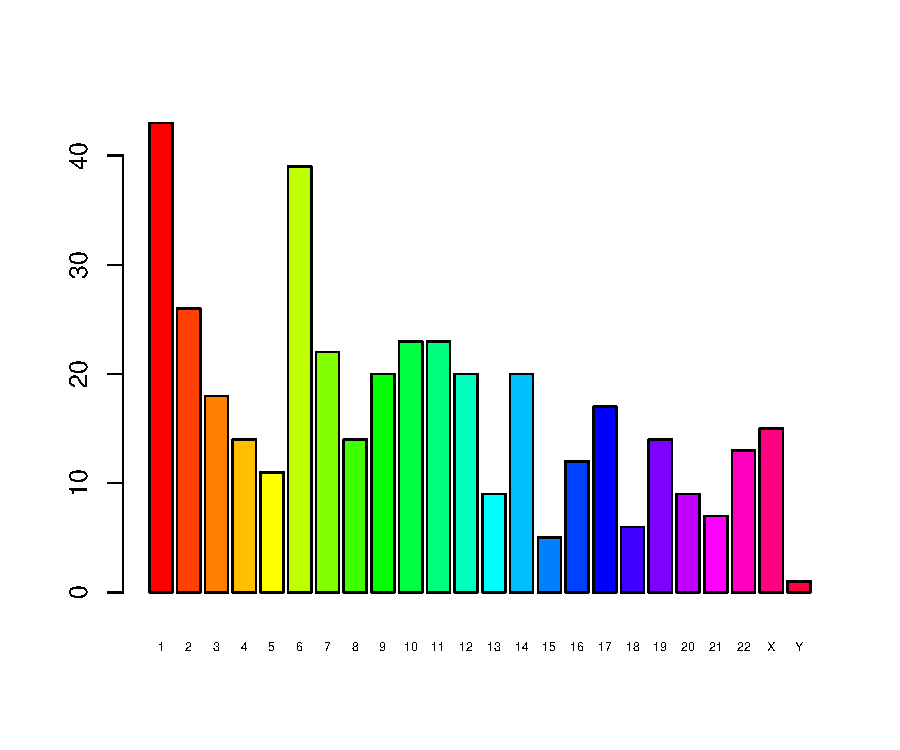
\includegraphics{plots/fig-017}
\end{frame}

\begin{frame}[allowframebreaks]
  \frametitle{Checking}
  \begin{itemize}
  \item Why did I use the \pl{sub} commands?
  \item Why did I use \pl{order} inside the \pl{barplot} call?
  \end{itemize}
\end{frame}

\begin{frame}[allowframebreaks, fragile]
  \frametitle{A sweet html table}
  \begin{itemize}
  \item Now lets assume that you want to show a table for the 400 genes in ALLsub to someone.
  \item Lets use the \pl{annaffy} package to create an html table:
\begin{Schunk}
\begin{Sinput}
> library("annaffy")
> anncols <- aaf.handler(chip = "hgu95av2.db")[c(1:3, 
+     8:9, 11:13)]
> anntable <- aafTableAnn(featureNames(ALLsub), 
+     "hgu95av2.db", anncols)
> saveHTML(anntable, "ALLsub.html", 
+     title = "The Features in ALLsub")
\end{Sinput}
\end{Schunk}
  \item We can open the html file directly from R using:
\begin{Schunk}
\begin{Sinput}
> localURL = file.path(getwd(), "ALLsub.html")
> browseURL(localURL)
\end{Sinput}
\end{Schunk}
  \item Open the html file :)
  \end{itemize}
\end{frame}

%%%%%%%%%%%%%%%%%%%%%%%%%%%%%%%%%%%%%%%%%%%%%%%%%%%%%%%%%%%%%%%%%%%%%%%%%%%
\section{Complications}

\begin{frame}[allowframebreaks, fragile]
  \frametitle{Multiple measurements}
  \begin{itemize}
  \item A big problem is that multiple probe sets can match to the same gene, which means that for some you have more measurements than for others. Also, alternative splicing can give you headaches.
  \item These R packages follow the ENCODE Project Consortium.
  \item Lets look at an example:
\begin{Schunk}
\begin{Sinput}
> probeSetsPerGene <- split(names(EG), 
+     EG)
> j <- probeSetsPerGene$"7013"
> j
\end{Sinput}
\begin{Soutput}
[1] "1329_s_at"  "1342_g_at" 
[3] "1361_at"    "32255_i_at"
[5] "32256_r_at" "32257_f_at"
[7] "32258_r_at"
\end{Soutput}
\end{Schunk}
  \item We found 7 probes matching to the same gene (EntrezGene ID 7013).
  \end{itemize}
\end{frame}


\begin{frame}[fragile, allowframebreaks]
  \frametitle{Example complication}
  Lets look at the expression values from 2 of them:
\begin{Schunk}
\begin{Sinput}
> plot(t(exprs(ALL_af4bcr)[j[c(1, 
+     7)], ]), asp = 1, pch = 16, 
+     col = ifelse(ALL_af4bcr$mol.biol == 
+         "ALL1/AF4", "black", "grey"))
\end{Sinput}
\end{Schunk}
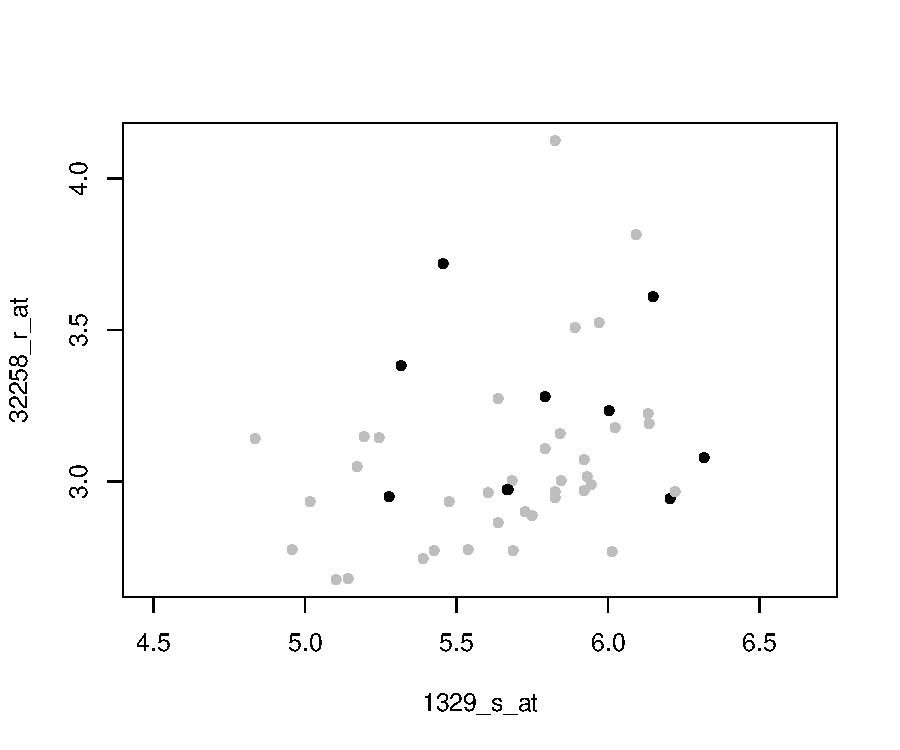
\includegraphics{plots/fig-021}
\end{frame}

\begin{frame}[fragile, allowframebreaks]
  \frametitle{A complicated plot}
  We now used a different trick to map the colors: the \BIOCfunction{ifelse} function. \\
  A better plot in this case is the heatmap using the \pl{lattice} function \BIOCfunction{levelplot}. Lets make one for the our gene 7013.
\begin{Schunk}
\begin{Sinput}
> library("lattice")
> mat <- exprs(ALL_af4bcr)[j, ]
> mat <- mat - rowMedians(mat)
> ro <- order.dendrogram(as.dendrogram(hclust(dist(mat))))
> co <- order.dendrogram(as.dendrogram(hclust(dist(t(mat)))))
> at <- seq(-1, 1, length = 21) * 
+     max(abs(mat))
> lp <- levelplot(t(mat[ro, co]), 
+     aspect = "fill", at = at, scales = list(x = list(rot = 90)), 
+     colorkey = list(space = "left"))
> print(lp)
\end{Sinput}
\end{Schunk}
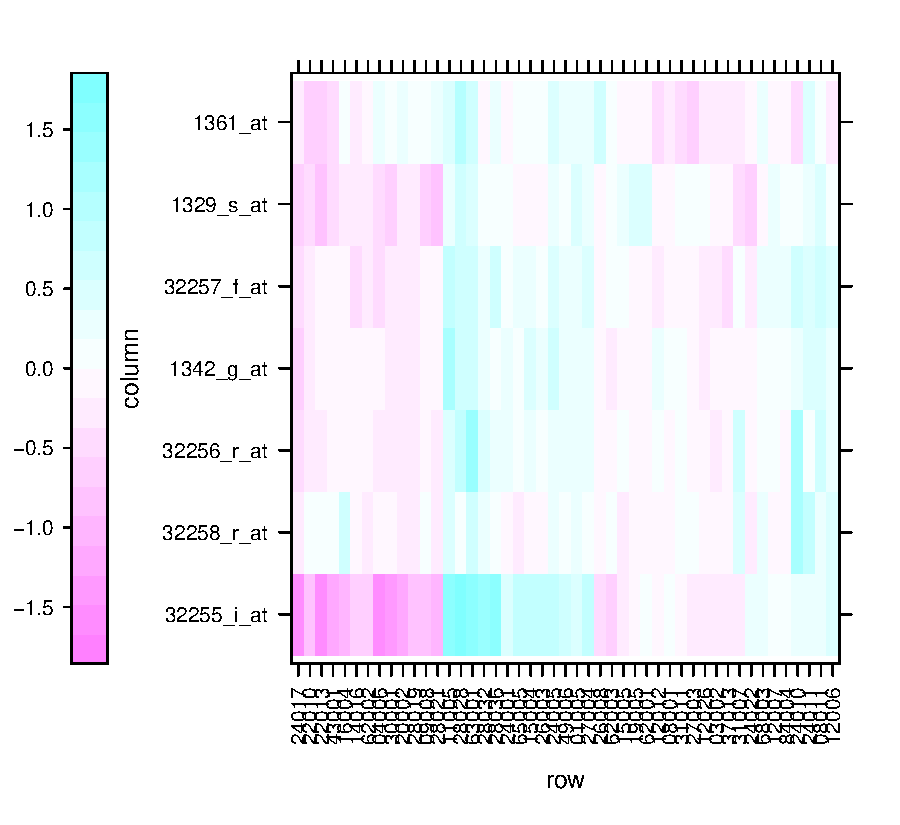
\includegraphics{plots/fig-022}
\end{frame}

%%%%%%%%%%%%%%%%%%%%%%%%%%%%%%%%%%%%%%%%%%%%%%%%%%%%%%%%%%%%%%%%%%%%%%%%%%%
\section{Some statistics}

\begin{frame}[allowframebreaks, fragile]
  \frametitle{chr}
  \begin{itemize}
  \item One of  the tests we can make now is to check for every chromosome, the low and high p values.
  \item To do so we can use \pl{chisq.test} and \pl{fisher.test}.
  \item First we need to create a data frame to map for every EntrezGene ID to which chromosome it belongs:
\begin{Schunk}
\begin{Sinput}
> ps_chr <- toTable(hgu95av2CHR)
> ps_eg <- toTable(hgu95av2ENTREZID)
> chr <- merge(ps_chr, ps_eg)
> dim(chr)
\end{Sinput}
\begin{Soutput}
[1] 11972     3
\end{Soutput}
\end{Schunk}
  \item We don't need the first column, so lets take it out:
\begin{Schunk}
\begin{Sinput}
> chr <- unique(chr[, colnames(chr) != 
+     "probe_id"])
> dim(chr)
\end{Sinput}
\begin{Soutput}
[1] 9009    2
\end{Soutput}
\begin{Sinput}
> head(chr)
\end{Sinput}
\begin{Soutput}
  chromosome gene_id
1         14    5875
2         16    5595
3          1    7075
4         10    1557
5         11     643
7          5    1843
\end{Soutput}
\end{Schunk}
  \item What problem do you notice? You might need to explore \pl{chr} in full.
  \end{itemize}
\end{frame}

\begin{frame}[allowframebreaks, fragile]
  \frametitle{Duplications}
  \begin{itemize}
  \item Look at this table:
\begin{Schunk}
\begin{Sinput}
> table(table(chr$gene_id))
\end{Sinput}
\begin{Soutput}
   1    2 
8985   12 
\end{Soutput}
\end{Schunk}
  \item Lets take out those complicated genes that have duplicated entries.
\begin{Schunk}
\begin{Sinput}
> chr <- chr[!duplicated(chr$gene_id), 
+     ]
\end{Sinput}
\end{Schunk}
  \end{itemize}
\end{frame}

\begin{frame}[allowframebreaks, fragile]
  \frametitle{Checking for association}
  \begin{itemize}
  \item Now we can do the a contigency table for the association between the EntrezGene ID with their chromosome mapping \alert{and} with being differently expressed.
  \item Lets re-use our EGsub object which had those differently expressed.
\begin{Schunk}
\begin{Sinput}
> isdiff <- chr$gene_id %in% EGsub
> tab <- table(isdiff, chr$chromosome)
> tab
\end{Sinput}
\begin{Soutput}
isdiff    1  10  11  12  13  14  15  16
  FALSE 898 304 498 474 150 271 256 366
  TRUE   43  23  23  20   9  20   5  12
       
isdiff   17  18  19   2  20  21  22   3
  FALSE 512 122 543 547 221  93 249 461
  TRUE   17   6  14  26   9   7  13  18
       
isdiff    4   5   6   7   8   9  Un   X
  FALSE 326 390 490 406 297 311   4 384
  TRUE   14  11  39  22  14  20   0  15
       
isdiff    Y
  FALSE  24
  TRUE    0
\end{Soutput}
\end{Schunk}
  \item Once we have this table, we can do a Fisher's exact test:
\begin{Schunk}
\begin{Sinput}
> fisher.test(tab, simulate.p.value = TRUE)
\end{Sinput}
\begin{Soutput}
	Fisher's Exact Test for Count Data
	with simulated p-value (based on
	2000 replicates)

data:  tab 
p-value = 0.01499
alternative hypothesis: two.sided 
\end{Soutput}
\end{Schunk}
  \item And a Chi squared test:
\begin{Schunk}
\begin{Sinput}
> chisq.test(tab)
\end{Sinput}
\begin{Soutput}
	Pearson's Chi-squared test

data:  tab 
X-squared = 42.2405, df = 24,
p-value = 0.01213
\end{Soutput}
\end{Schunk}
  \item What can we conclude?
  \end{itemize}
\end{frame}

\begin{frame}[allowframebreaks, fragile]
  \frametitle{Strand bias}
  \begin{itemize}
  \item We can also check for where the genes are located, what other genes are nearby, grouping genes by location before another test, \ldots
  \item Lets check if our differentially expressed genes are on the same strand:
\begin{Schunk}
\begin{Sinput}
> chrloc <- toTable(hgu95av2CHRLOC[featureNames(ALLsub)])
> head(chrloc)
\end{Sinput}
\begin{Soutput}
  probe_id start_location Chromosome
1  1635_at      132579088          9
2  1635_at      132700651          9
3 39329_at      -68410592         14
4 40797_at      -56675801         15
5 33800_at       -3952652         16
6 34777_at       10283217         11
\end{Soutput}
\end{Schunk}
  \item Alternative splicing will give us some problems:
\begin{Schunk}
\begin{Sinput}
> table(table(chrloc$probe_id))
\end{Sinput}
\begin{Soutput}
  1   2   3   4   5   6   9 
285  66  33   9   3   3   1 
\end{Soutput}
\end{Schunk}
  \item Lets collapse the information so that we only record the strand, which should be the same even if there is alternative splicing:
\begin{Schunk}
\begin{Sinput}
> strds <- with(chrloc, unique(cbind(probe_id, 
+     sign(start_location))))
> table(strds[, 2])
\end{Sinput}
\begin{Soutput}
 -1   1 
194 206 
\end{Soutput}
\end{Schunk}
  \item What do we conclude?
  \end{itemize}
\end{frame}

%%%%%%%%%%%%%%%%%%%%%%%%%%%%%%%%%%%%%%%%%%%%%%%%%%%%%%%%%%%%%%%%%%%%%%%%%%%
\section{GO}

\begin{frame}[allowframebreaks]
  \frametitle{Quick review}
  \begin{itemize}
  \item GO, short for Gene Ontology, classifies genes products according to
  \begin{enumerate}
  \item Molecular function
  \item Biological process
  \item Cellular component
  \end{enumerate}
  \item GO terms are represented in a graph where there are two types of relationships:
  \begin{enumerate}
  \item is as
  \item part of
  \end{enumerate}
  \item To facilitate the mapping, GO terms are identified in 7 numbers. 
  \item All the descendants of a given GO term are called \emph{offspring}. The immediate ones are called \emph{children}.
  \item All the parental GO terms are called \emph{ancestor}.
  \end{itemize}
\end{frame}

\begin{frame}[allowframebreaks, fragile]
  \frametitle{GO.db}
  \begin{itemize}
  \item In R, the package \pl{GO.db} enables us to browse the GO tree:
\begin{Schunk}
\begin{Sinput}
> library("GO.db")
> as.list(GOMFCHILDREN["GO:0008094"])
\end{Sinput}
\begin{Soutput}
$`GO:0008094`
         isa          isa          isa 
"GO:0004003" "GO:0015616" "GO:0033170" 
         isa          isa          isa 
"GO:0033676" "GO:0033680" "GO:0043142" 
\end{Soutput}
\begin{Sinput}
> as.list(GOMFOFFSPRING["GO:0008094"])
\end{Sinput}
\begin{Soutput}
$`GO:0008094`
 [1] "GO:0003689" "GO:0004003"
 [3] "GO:0015616" "GO:0017116"
 [5] "GO:0033170" "GO:0033676"
 [7] "GO:0033680" "GO:0033681"
 [9] "GO:0033682" "GO:0043140"
[11] "GO:0043141" "GO:0043142"
\end{Soutput}
\end{Schunk}
  \end{itemize}
\end{frame}

\begin{frame}[allowframebreaks, fragile]
  \frametitle{Hyper Geometric GO test}
  \begin{itemize}
  \item The packages \alert{annotate} and \alert{GOstats} are the basic ones to carry out GO analysis.
  \item Other related packages are \BIOCfunction{topGO} and \BIOCfunction{goTools}.
  \item Lets make the basic GO test. We want to compare the frequency of a GO term on a subset versus the frequency of the same GO term on the overall universe.
  \item Things get complicated because some GO terms have more offspring than others\ldots
  \item Lets do the test (actually, lots of tests) for our data:
\begin{Schunk}
\begin{Sinput}
> library("GOstats")
> affyUniverse <- featureNames(ALLfilt_af4bcr)
> uniId <- hgu95av2ENTREZID[affyUniverse]
> entrezUniverse <- unique(as.character(uniId))
> params <- new("GOHyperGParams", 
+     geneIds = EGsub, universeGeneIds = entrezUniverse, 
+     annotation = "hgu95av2", ontology = "BP", 
+     pvalueCutoff = 0.001, conditional = FALSE, 
+     testDirection = "over")
\end{Sinput}
\end{Schunk}
  \item After building up all the parameters we can now make the actual test:
\begin{Schunk}
\begin{Sinput}
> myhyper <- hyperGTest(params)
\end{Sinput}
\end{Schunk}
  \end{itemize}
\end{frame}

\begin{frame}[fragile, allowframebreaks]
  \frametitle{P values}
  We didn't adjust our p values as it can complicated. Instead, lets visualize the histogram:
\begin{Schunk}
\begin{Sinput}
> hist(pvalues(myhyper), breaks = 50, 
+     col = "mistyrose")
\end{Sinput}
\end{Schunk}
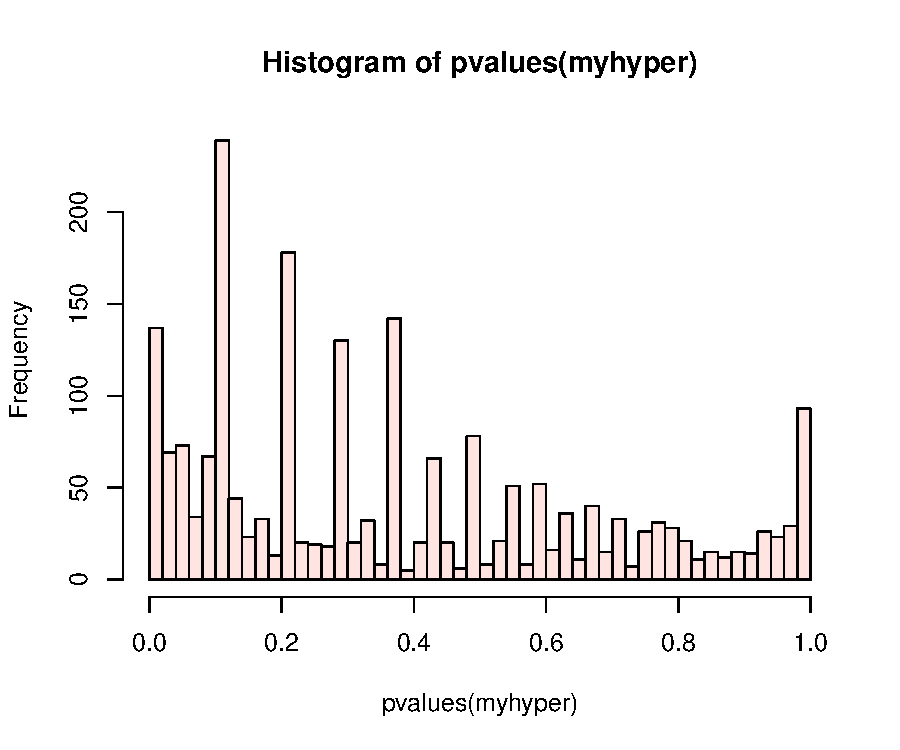
\includegraphics{plots/fig-036}
\end{frame}

\begin{frame}[allowframebreaks, fragile]
  \frametitle{Summary for myhyper}
  \begin{itemize}
  \item As you can notice, we have a peak on the left side. Meaning that we have several low p values.
  \item Lets look deeper into the results from our test: \scriptsize
\begin{Schunk}
\begin{Sinput}
> sum <- summary(myhyper, p = 0.001)
> head(sum)
\end{Sinput}
\begin{Soutput}
      GOBPID       Pvalue OddsRatio
1 GO:0007154 3.683084e-09  1.903807
2 GO:0007165 9.991034e-09  1.883483
3 GO:0006955 3.396946e-07  2.416384
4 GO:0019882 8.991223e-07  6.479221
5 GO:0002376 5.214422e-06  1.998862
6 GO:0006687 9.127024e-06 50.939086
    ExpCount Count Size
1 116.390817   168 1090
2 109.663641   159 1027
3  27.442605    54  257
4   3.737320    15   35
5  39.829151    67  373
6   0.747464     6    7
                                 Term
1                  cell communication
2                 signal transduction
3                     immune response
4 antigen processing and presentation
5               immune system process
6 glycosphingolipid metabolic process
\end{Soutput}
\end{Schunk}
  \normalsize
  \item What do you notice? What can you conclude?
  \end{itemize}
\end{frame}

\begin{frame}[allowframebreaks, fragile]
  \frametitle{Longer definitions}
  \begin{itemize}
  \item Even though the GO term definition is better than the GO ID, it is not sufficient.
  \item So lets take a look at the actual definitions using the \pl{GO.db} package:
\begin{Schunk}
\begin{Sinput}
> GOTERM[["GO:0032945"]]
\end{Sinput}
\begin{Soutput}
GOID: GO:0032945
Term: negative regulation of
    mononuclear cell proliferation
Ontology: BP
Definition: Any process that stops,
    prevents or reduces the
    frequency, rate or extent of
    mononuclear cell proliferation.
Synonym: negative regulation of
    PBMC proliferation
Synonym: negative regulation of
    peripheral blood mononuclear
    cell proliferation
\end{Soutput}
\end{Schunk}
  \end{itemize}
\end{frame}

%%%%%%%%%%%%%%%%%%%%%%%%%%%%%%%%%%%%%%%%%%%%%%%%%%%%%%%%%%%%%%%%%%%%%%%%%%%
\section{More on GO}

\begin{frame}[allowframebreaks]
  \frametitle{biomaRt}
  \begin{itemize}
  \item Remember that you can use \BIOCfunction{biomaRt} to get GO IDs or to use them as a query and get more information on your genes / proteins.
  \item For instance, take a look at the \BIOCfunction{getGo} function.
  \item You can find GO IDs from \pl{biomaRt} in PFAM, Prosite, and InterPro besides the usual, ENSEMBL.
  \end{itemize}
\end{frame}

\begin{frame}[allowframebreaks]
  \frametitle{SQL based packages}
  \begin{itemize}
  \item Several packages, for example hgu133a and hgu95av2 were changed from being \emph{environment} based to SQL based packages.
  \item They did this change to facilitate mapping between different identifiers.
  \item This was specially useful in cases where you have incomplete data.
  \item Plus it made everything faster :)
  \end{itemize}
\end{frame}

\begin{frame}[allowframebreaks, fragile]
  \frametitle{An example:}
  \begin{itemize}
  \item Old way:
\begin{Schunk}
\begin{Sinput}
> goCats <- unlist(eapply(GOTERM, 
+     Ontology))
> old <- table(goCats)[c("BP", "CC", 
+     "MF")]
\end{Sinput}
\end{Schunk}
  \item New way \alert{WAY faster}:  
\begin{Schunk}
\begin{Sinput}
> query <- "select ontology from go_term"
> goCats <- dbGetQuery(GO_dbconn(), 
+     query)
> new <- table(goCats)[c("BP", "CC", 
+     "MF")]
\end{Sinput}
\end{Schunk}
  \item Comparing:
\begin{Schunk}
\begin{Sinput}
> identical(old, new)
\end{Sinput}
\begin{Soutput}
[1] TRUE
\end{Soutput}
\end{Schunk}
  \end{itemize}
\end{frame}

%%%%%%%%%%%%%%%%%%%%%%%%%%%%%%%%%%%%%%%%%%%%%%%%%%%%%%%%%%%%%%%%%%%%%%%%%%%
\section{Credits}

\begin{frame}[allowframebreaks]
  \frametitle{Credits}
  \begin{itemize}
  \item \BIOCfunction{Bioconductor Case Studies} by Florian Hahne, Wolfgang Huber, Robert Gentleman and Seth Falcon.
  \item Specially chapter 8.
  \end{itemize}
\end{frame}

%%%%%%%%%%%%%%%%%%%%%%%%%%%%%%%%%%%%%%%%%%%%%%%%%%%%%%%%%%%%%%%%%%%%%%%%%%%
\section{Homework}
\begin{frame}[allowframebreaks]
  \frametitle{Homework}
  \begin{itemize}
  \item Choose a different EntrezGene ID (not 7013) that has different probes.
  \item Make a scatterplot compairing the expression values from two probe sets.
  \item Make the heatmap showing all the probe sets.
  \item Add your conclusions.
  \end{itemize}
\end{frame}

\begin{frame}[allowframebreaks, fragile]
  \frametitle{SessionInfo} \scriptsize
\begin{Schunk}
\begin{Sinput}
> sessionInfo()
\end{Sinput}
\begin{Soutput}
R version 2.9.0 (2009-04-17) 
i386-pc-mingw32 

locale:
LC_COLLATE=English_United States.1252;LC_CTYPE=English_United States.1252;LC_MONETARY=English_United States.1252;LC_NUMERIC=C;LC_TIME=English_United States.1252

attached base packages:
[1] stats     graphics  grDevices
[4] utils     datasets  methods  
[7] base     

other attached packages:
 [1] GOstats_2.10.0     
 [2] graph_1.22.2       
 [3] Category_2.10.1    
 [4] lattice_0.17-22    
 [5] annaffy_1.16.0     
 [6] KEGG.db_2.2.11     
 [7] GO.db_2.2.11       
 [8] annotate_1.22.0    
 [9] hgu95av2.db_2.2.12 
[10] RSQLite_0.7-1      
[11] DBI_0.2-4          
[12] AnnotationDbi_1.6.0
[13] genefilter_1.24.3  
[14] ALL_1.4.5          
[15] Biobase_2.4.1      

loaded via a namespace (and not attached):
[1] grid_2.9.0      GSEABase_1.6.1 
[3] RBGL_1.20.0     splines_2.9.0  
[5] survival_2.35-4 tools_2.9.0    
[7] XML_2.5-1       xtable_1.5-5   
\end{Soutput}
\end{Schunk}
\end{frame}

\end{document}

